%%=============================================================================
%% De eerste hulp assistent
%%=============================================================================

\chapter{De eerste hulp assistent}
\label{ch:De eerste hulp assistent}

\section{De gekozen assistent}
De applicatie zal ontwikkeld worden voor Google Assistant. Met de komst van een Belgische variant lijkt Google nu de eerste te zijn die de intrede zal maken in België voor het grote publiek. Meer hierover is te lezen onder \ref{ss:de spraakassistenten van nu}.
Uit het vergelijkende onderzoek is gebleken dat de spraakkwaliteit bij de Nederlandstalige Google Assistant aanzienlijk lager ligt dan bij zijn Engelse variant en Alexa. Toch wordt er voor deze assistent gekozen omdat het spreken van de Nederlandse taal een beslissende factor is in de keuze van de te gebruiken assistent.

\section{De werking van Google Assistant}
\begin{figure}[h]
    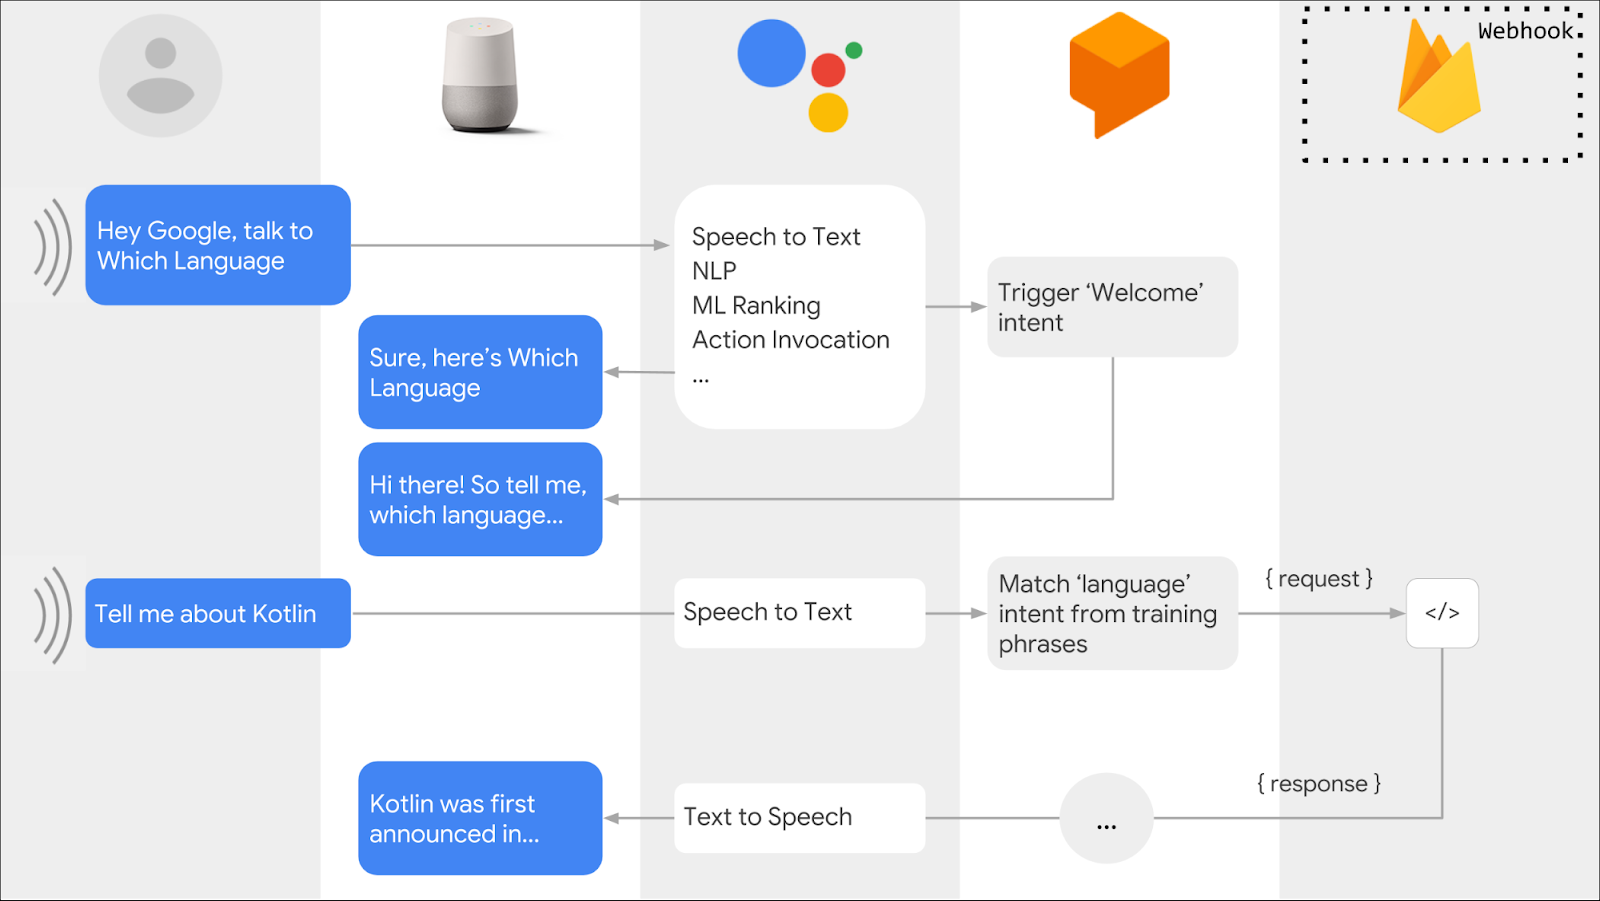
\includegraphics[width=0.7\linewidth]{img/gaflow}
    \caption{De technische architectuur van Google Assistant \autocite{Brandt2018}}
    \label{fig:gaflow}
\end{figure}

Een applicatie voor Google Assistant wordt een action genoemd. De gebruiker kan actions openen door het simpelweg te vragen met een eenvoudig commando als 'praat met ..'. De assistent gaat controleren of de action bestaat en zal ze invoceren. Afhankelijk van de invocatie zal er een intent worden gestart in DialogFlow. DialogFlow is een online tool die kan geïntegreerd worden met de action en die instaat voor de conversatie interface. Een intent is een verzameling van de mogelijke invoer van de gebruiker voor één antwoord. In een intent worden trainingsvragen geschreven die DialogFlow helpen om de juiste intent te triggeren. Wanneer een intent geen vast antwoord kan geven wordt een webhook, een koppeling naar een programma dat geschreven is door de ontwikkelaar, gebruikt om de extra functionaliteit af te handelen. Denk maar aan het berekenen van het BMI bij een 'bereken BMI'-action of het ophalen van data uit een API.
Wat belangrijk zal zijn bij de 'eerste hulp'-action is dat hij kan gestart worden door een combinatie van de actie naam en een invocatiezin, vb. praat met EHBO hulp want mijn vader is flauwgevallen. Hierdoor wordt met één zin de action gestart en wordt door de invocatiezin de intent gestart die de juiste instructies zal geven. We gaan even meer in detail bekijken hoe de de 'eerste hulp'-action er kan uitzien.

\section{De werking van de applicatie}
De functionaliteit is gebaseerd op de werking van de mobiele applicatie. Meer hierover kun je vinden onder \ref{ss:de vlaamse ehbo-app van het rode kruis}. De functionaliteit is gevisualiseerd met een flowchart.

\begin{figure}[h]
    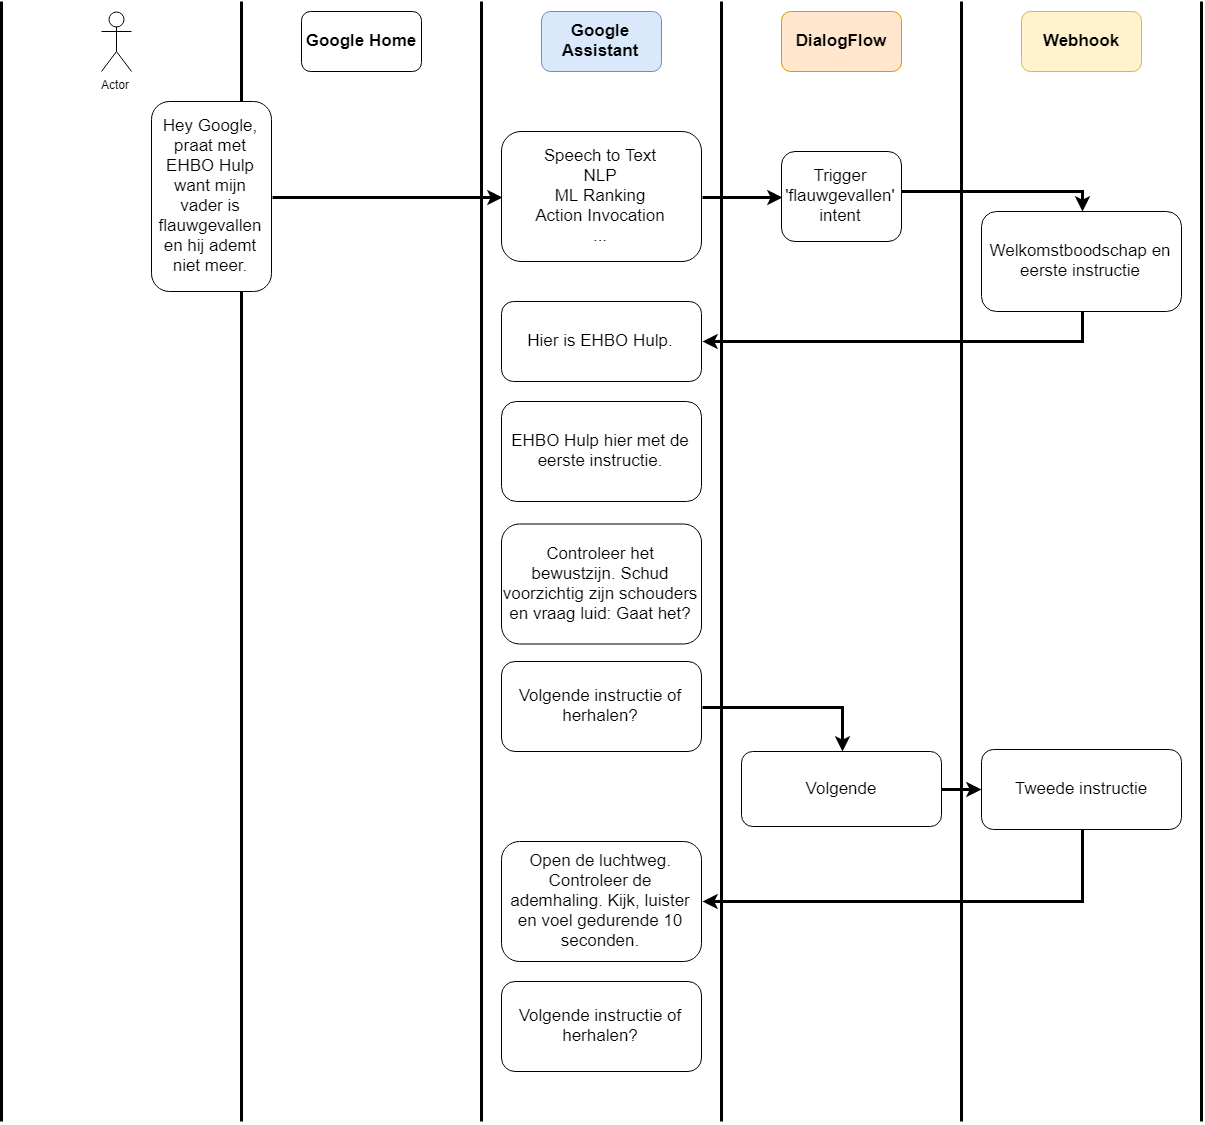
\includegraphics[width=0.7\linewidth]{img/gaflowehbo}
    \caption{De werking van de 'EHBO Hulp'-action}
    \label{fig:gaflowehbo}
\end{figure}

\section{De ontwikkeling van de applicatie}
De ontwikkeling van de applicatie is nog niet gestart tijdens het schrijven van deze bachelorproef. De plannen zijn er om in de eerste weken na het indienen een eerste versie te ontwikkelen. Het is de bedoeling dat er feedback gevraagd wordt aan willekeurige gebruikers en bij voorkeur ook aan medewerkers van het Rode Kruis. Indien de feedback positief blijkt te zijn kan er geopteerd worden om de applicatie verder uit te werken.


